\documentclass[10pt]{article}
\usepackage{times}
\usepackage{graphicx}
\title{Healthcare-ML: Clinical Risk Modeling with API Data}
\author{Jibran Kazi (JK)}
\date{October 2025}
\begin{document}
\maketitle
\begin{abstract}
We present a reproducible, API-driven clinical risk pipeline with AUROC/AUPRC evaluation and calibration analysis.
\end{abstract}
\section{Data \& Method}
We load a public medical dataset via API (fallback to scikit-learn breast cancer), train a calibrated classifier, and evaluate.
\section{Results}
\begin{tabular}{l r}
\hline
Metric & Value \\ \hline
AUROC & 0.9982 \\ 
AUPRC & 0.9989 \\ \hline
\end{tabular}

\begin{figure}[h]
\centering
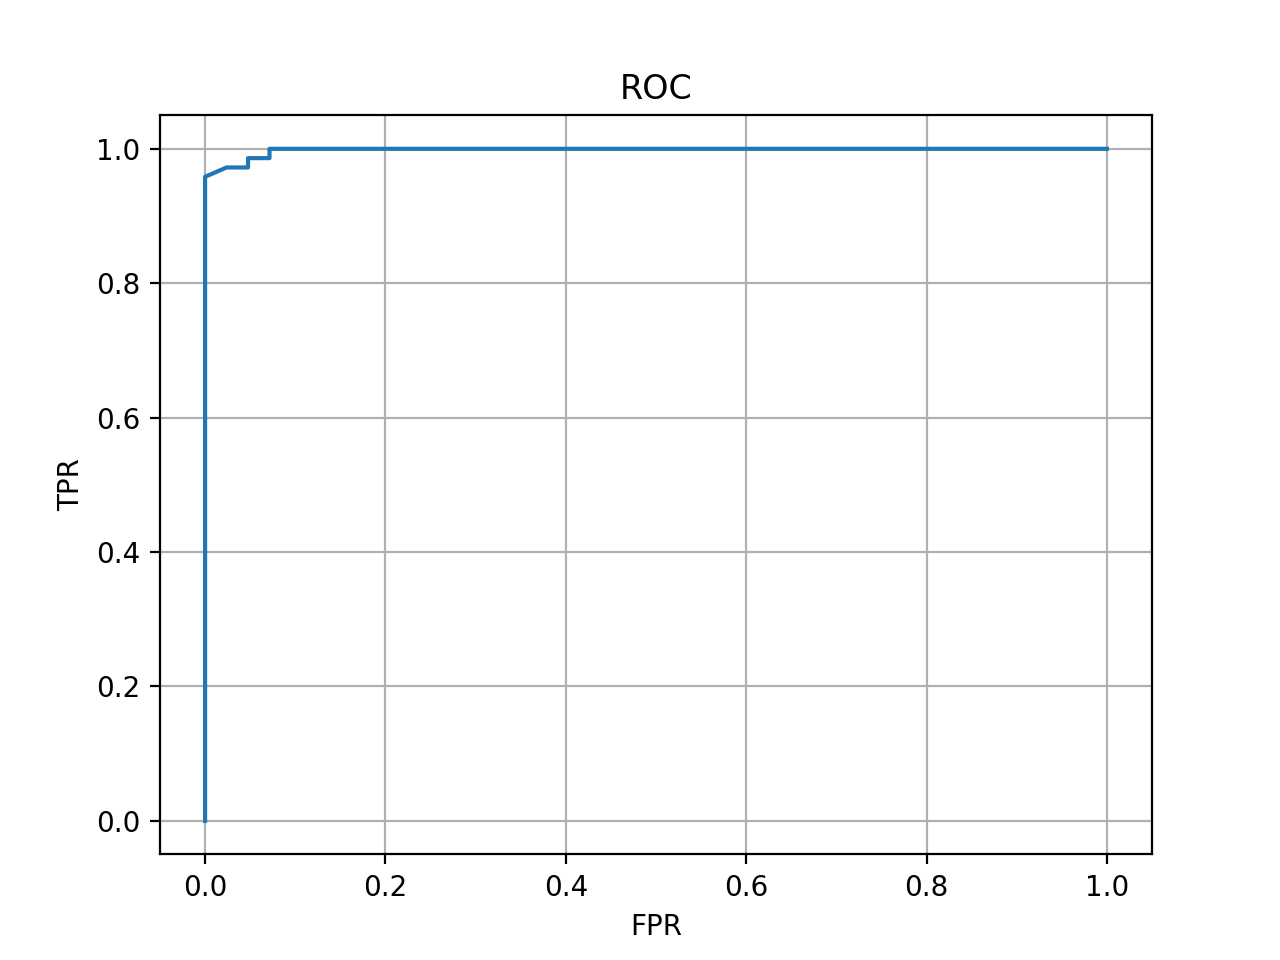
\includegraphics[width=0.45\linewidth]{figures/roc.png}
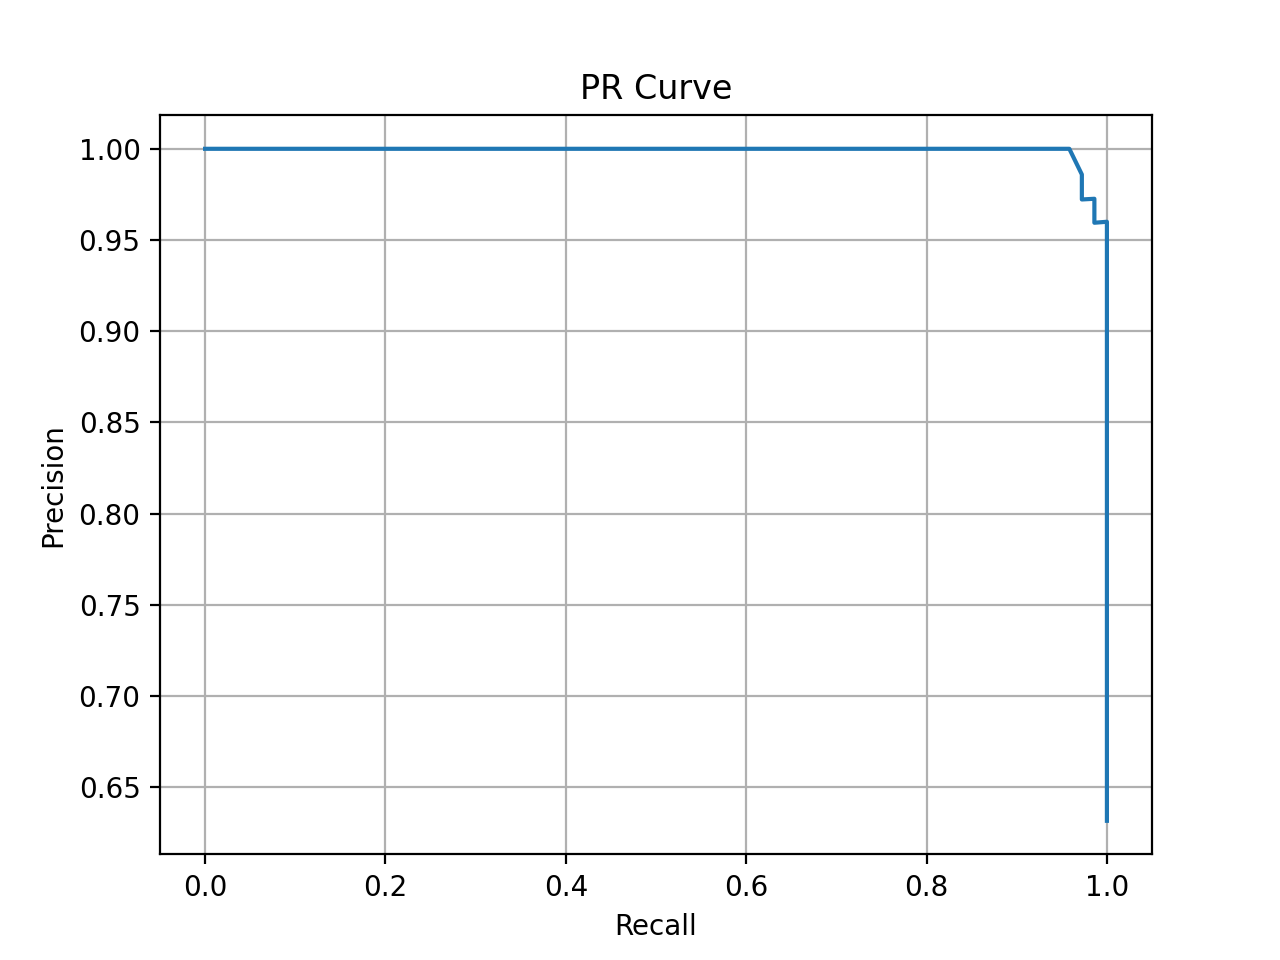
\includegraphics[width=0.45\linewidth]{figures/pr.png}
\caption{ROC and PR curves.}
\end{figure}
\begin{figure}[h]
\centering
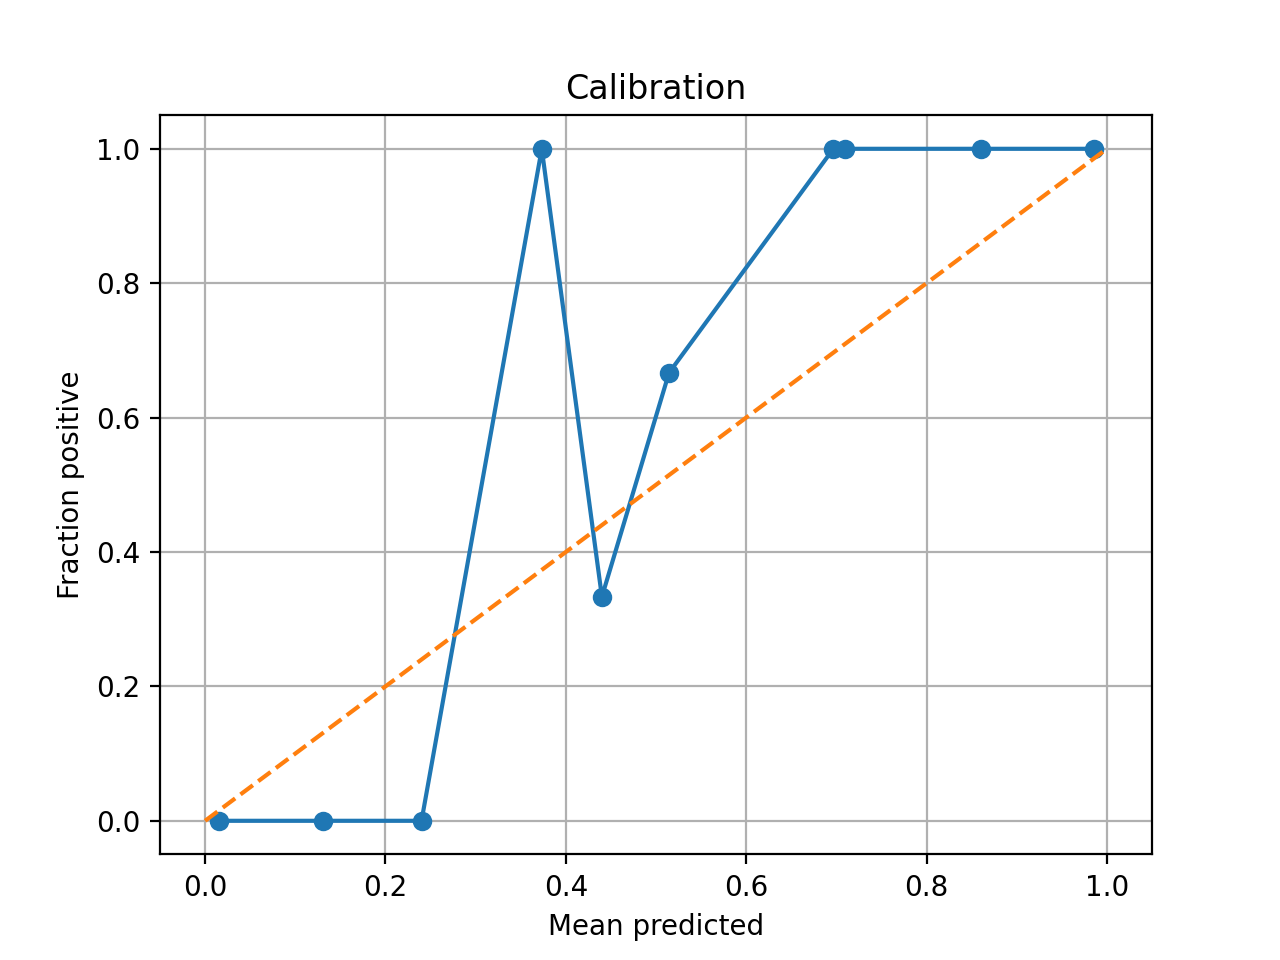
\includegraphics[width=0.6\linewidth]{figures/calibration.png}
\caption{Calibration curve.}
\end{figure}
\end{document}
